\section{Layout}

The layout is arranged as a column of transistors stacked one on top of each other as shown in the next diagram, where the names of the components are in accordance with those in Fig 1. 

The capacitors are placed on top of the transistors. They have a size of 12x4 $\mu m$ which corresponds to the maximum length/width ratio and the minimum width. This makes the design as compact as possible. In total, the pixel is 506 $\mu m$ long including the 10 $\mu m$ long photodiode. The design is made for a pixel pitch of 6.4 $\mu m$, although the final pitch is 8.6 $\mu m$ due to an AM spacing rule that did not show up in our preliminary analysis. 

The circuit is divided into the pixel circuit (bottom) and the digital reset circuit (top) to avoid interference between digital and analogue parts. Within the pixel circuit, there is a division between an nFET area and a pFET area which has a common n-well.

The transistors that had a W/L ratio of 6/2 have been made to have 3 fingers to better fit the design and make them square, which is the shape less sensitive to mismatch. 

As we move from the phodiode up to the other end of the pixel, we first find the transistors that operate with the photocurrent (Mn, Mcas and Mfb). These are placed closest to the photodiode to minimize resistive losses and addition of noise, as the photocurrent will be small. Mpr, which connects to these transistors is also as close as possible within the n-well. 
We then find the three inverters, which are placed in such a way that the distance between their n and p transistors is the same for the three of them. At the end of the pixel circuit we find the source follower composed of Mb2 and Msf which, although it is also connected to the transistors at the bottom, the connection is only to the gate so there won't be current flowing. 
Finally, there is the reset circuit. 

\makebox{
	\parbox[c]{1.3cm}{
		\framebox[1.3cm][c]{\(M_{ref}\)} \par
		\framebox[1.3cm][c]{\(M_{RA}\)} \par
		\framebox[1.3cm][c]{\(M_{CA}\)} \par
		\framebox[0.6cm][c]{\(M_{gr}\)} 
		\framebox[0.6cm][c]{\(M_{r}\)} \par
		\begin{center}
			...
		\end{center}	
		\framebox[1.3cm][c]{\(M_{b2}\)} \par	
		\framebox[1.3cm][c]{\(M_{sf}\)} \par
		\framebox[1.3cm][c]{\(M_{dp}\)} \par
		\framebox[1.3cm][c]{\(M_{ONp}\)} \par
		\framebox[1.3cm][c]{\(M_{OFFp}\)} \par
		\framebox[1.3cm][c]{\(M_{pr}\)} \par
		\framebox[1.3cm][c]{\(M_{dn}\)} \par
		\framebox[1.3cm][c]{\(M_{ONn}\)} \par
		\framebox[1.3cm][c]{\(M_{OFFn}\)} \par
		\framebox[1.3cm][c]{\(M_{fb}\)} \par
		\framebox[1.3cm][c]{\(M_{cas}\)} \par
		\framebox[1.3cm][c]{\(M_n\)} \par
		\framebox[1.3cm][c]{\(D\)} \par	
	}
}

The power lines run vertically along the pixel in wider metal 3 paths. The biases for the transistors also run along the pixel, which we now realize is an unnecessary complication, as they should just run horizontally across pixels at the position where they are used. 

Metals 1 to 4 are used for the connexions. 
Substrate or well contacts are placed every two or three transistors. 

\begin{figure}
	\center
	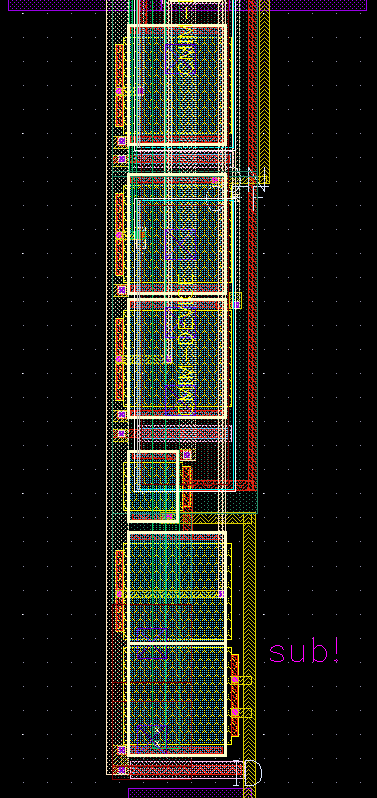
\includegraphics{pixel1.png}
	\caption{Pixel nFETs. From bottom to top, transistors $M_n, M_{cas}, M_{fb}, M_{OFFn}, M_{ONn}$ and $M_{dn}$. The path on the left is ground, vdd runs through the middle.}
	\label{uno}
\end{figure}

\begin{figure}
	\center
	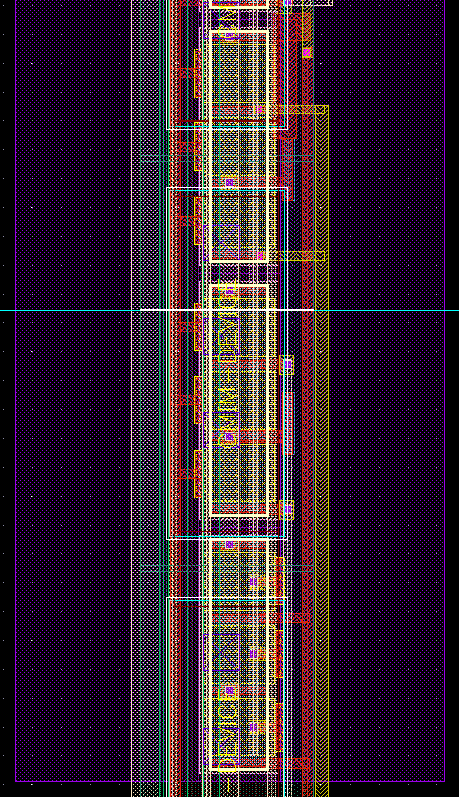
\includegraphics{pixel2.png}
	\caption{Pixel pFETS (I). From bottom to top, transistors $M_{pr}, M_{OFFp}$ and $M_{ONp}$.}
	\label{dos}
\end{figure}

\begin{figure}
	\center
	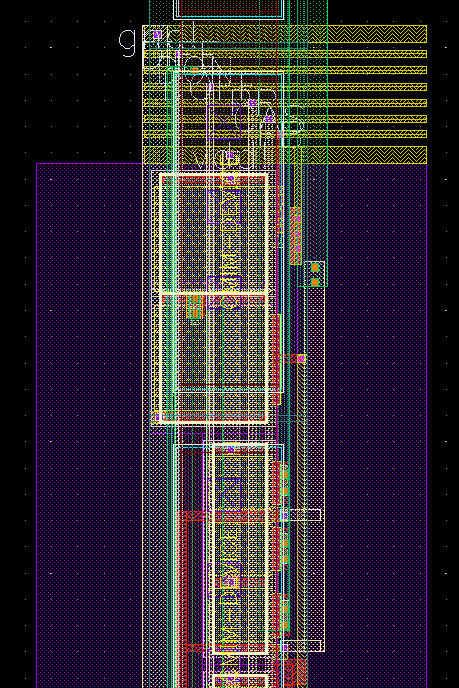
\includegraphics{pixel3.png}
	\caption{Pixel pFETS (II). From bottom to top, transistors $M_{dp}, M_{sf}$ and $M_{b2}$.}
	\label{tres}
\end{figure}

\begin{figure}
	\center
	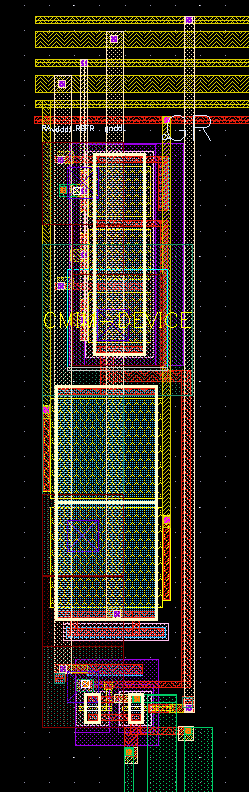
\includegraphics{pixel4.png}
	\caption{Reset circuit. From bottom to top, transistors $M_{gr}$ and $M_{r}$, $M_{CA}, M_{RA}$ and $M_{ref}$.}
	\label{cuatro}
\end{figure}
